\section{Calorimetry}

\makelabheader %(Space for student name, etc., defined in master.tex)

\bigskip
\textbf{Objectives}
\begin{itemize}[nosep]%[itemsep=1pt]%
\item To learn to use a method for measuring heat called calorimetry.
\item To use calorimetry to determine the specific heat of aluminum and
the heat of fusion of ice.
\end{itemize}

\bigskip
\textbf{Apparatus}

\begin{center}
\begin{tabular}{lll}
\textbullet \  Hypsometer    & \hspace{0.25in}\textbullet \  Calorimeter         & \hspace{0.25in}\textbullet \  Safety goggles \\
\textbullet \  Hot plate     & \hspace{0.25in}\textbullet \  Temperature probe   & \hspace{0.25in}\textbullet \  Compact scale (for measuring masses) \\
\textbullet \  Metal pellets & \hspace{0.25in}\textbullet \  Glass stirring rod  & \hspace{0.25in}\textbullet \  \textit{Capstone} software (\filename{Calorimetry.cap}) \\
\textbullet \  Plastic beaker& \hspace{0.25in}\textbullet \  Pasco 550 Interface & \hspace{0.25in} \\
\textbullet \  Ice           & \hspace{0.25in}\textbullet \  Clamp and stand     & \hspace{0.25in} \\
\end{tabular}
% \begin{tabular}{llll}
% \textbullet \  Hypsometer    &\textbullet \  Ice                &\textbullet \  Pasco 550 Interface                            & \textbullet \ Safety goggles   \\[2pt]
% \textbullet \  Hot plate     &\textbullet \  Calorimeter        &\textbullet \  Clamp and stand                                &  \\[2pt]
% \textbullet \  Metal pellets &\textbullet \  Temperature probe  &\textbullet \  \textit{Capstone} (\filename{Calorimetry.cap}) &  \\[2pt]
% \textbullet \  Plastic beaker&\textbullet \  Glass stirring rod &\textbullet \  Compact scale (for measuring masses)           &  \\
% \end{tabular}
\end{center}

\begin{center}
\begin{tabular}{ccc}
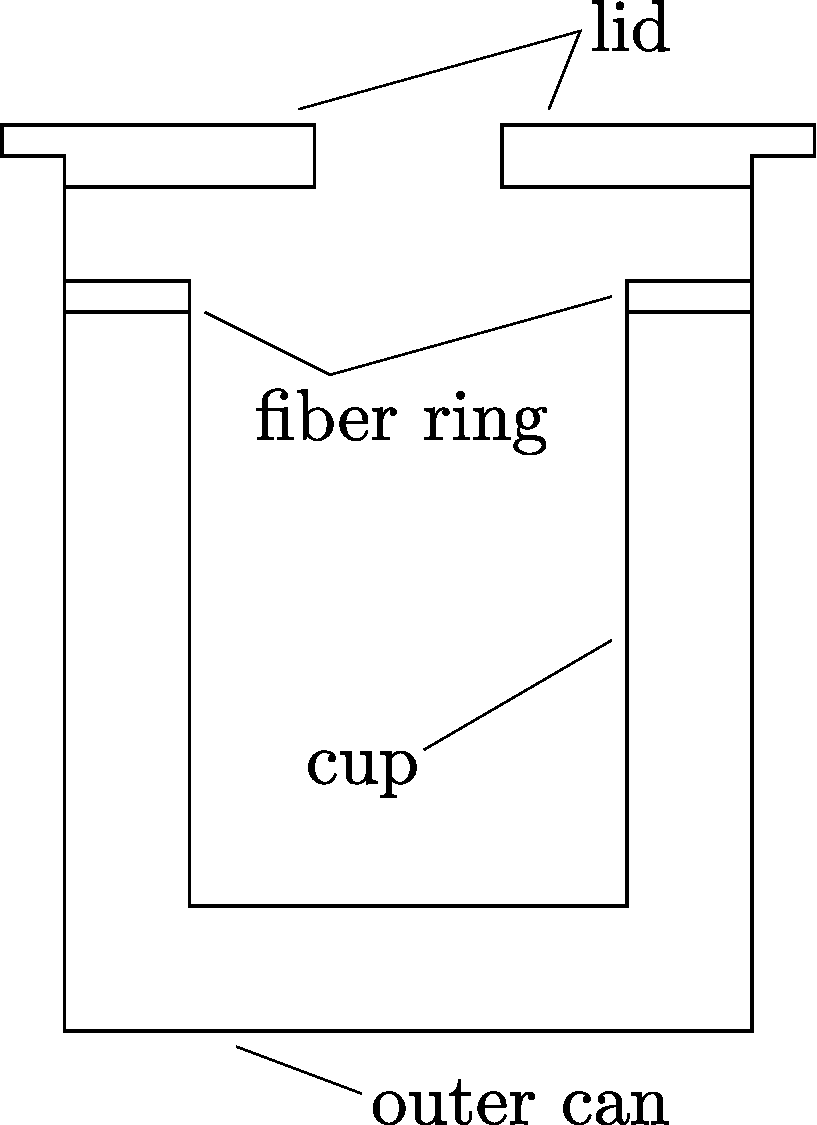
\includegraphics[height=3.0in]{calorimetry/calorimeter1.pdf} & \hspace{0.6in} & 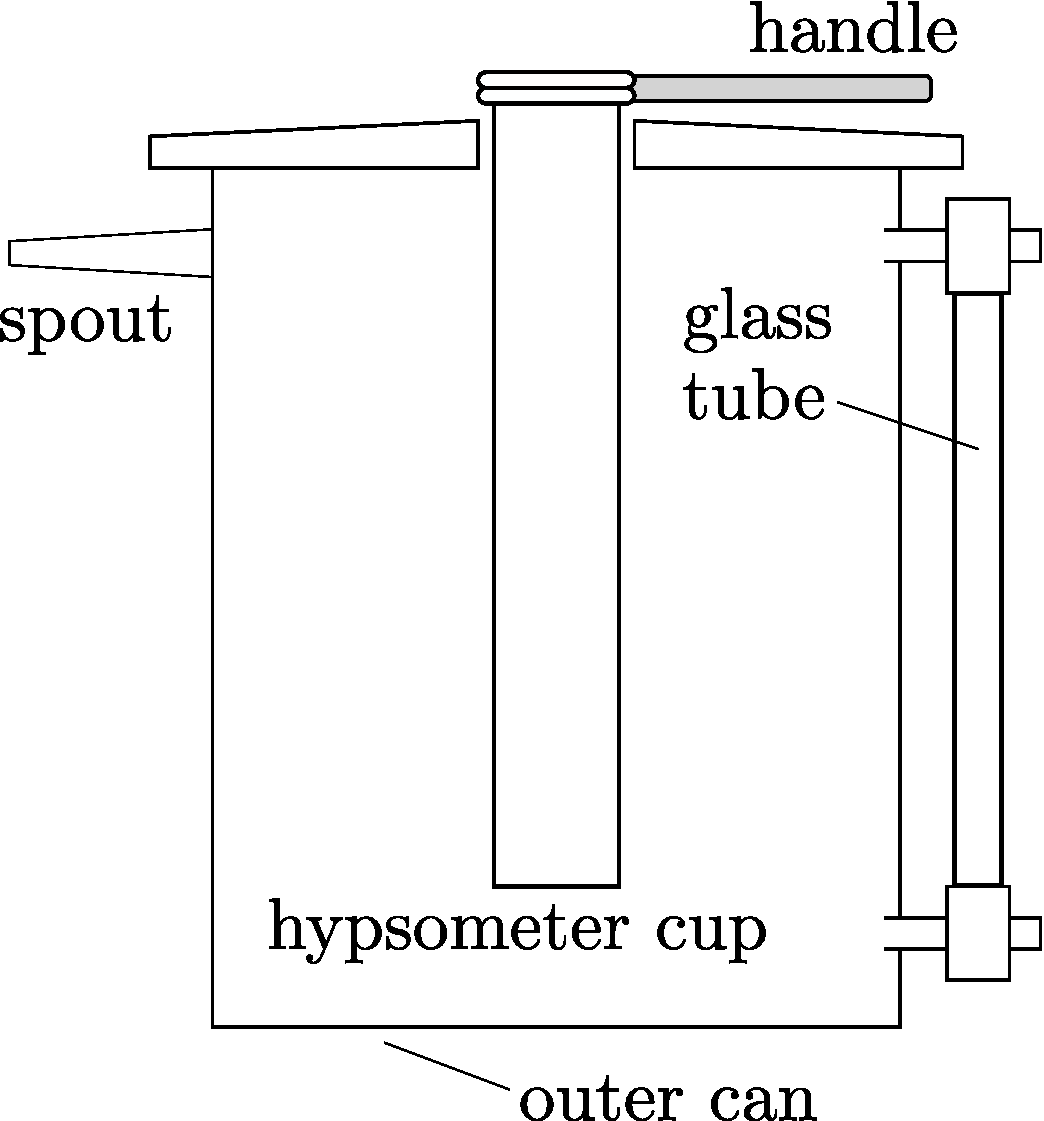
\includegraphics[height=3.0in]{calorimetry/hypsometer1.pdf} \\[5pt]
\LARGE Calorimeter                                           &                & \LARGE Hypsometer  \\
\end{tabular}
\end{center}

\bigskip
\textbf{Introduction} 

Calorimetry is a method for measuring heat. As applied in this experiment,
the method involves the mixing together of substances initially at
two different temperatures. The substances at the higher temperature
lose heat and the substances at the lower temperature gain heat until
thermal equilibrium is reached.

%\textbf{Experimental Equipment} 

A calorimeter, shown in the left-hand side of the figure, is used in this experiment
to minimize the exchange of heat between the system and the surroundings.
The inner calorimeter cup is thermally insulated from the surroundings
by suspending it on a ring of material with low heat conductivity
and surrounding it with a layer of air. Also the cup is shiny to minimize
radiation loss. Hence, if the mixture of substances is placed inside
the calorimeter cup, the heat lost to or gained from the surroundings
can be ignored, and the above relationship can be used. The only part
of the calorimeter which is involved in the calculation is the inner
calorimeter cup which contains water and in which an exchange of heat
between the hot and cold bodies takes place. The cup will undergo
the same temperature change as the contained water. Of course, an
instrument will have to be introduced to measure the temperature of
the system, but the heat gained or lost by the instrument is small
and can be ignored.

\pagebreak[3]

\textbf{Activity 1: Statement of Conservation of Energy}

If no heat is transferred to the surroundings, what is the relationship
between the heat lost by the substances initially at high temperature
and the heat gained by the substances initially at low temperature?
Note: This is simply a statement of conservation of energy.
\answerspace{15mm}

\textbf{Activity 2: Specific Heat of a Metal}

(a) Fill the hypsometer (boiler, shown in the right-hand side of the figure) 
at least half full of water and start heating the water. 
To avoid evaporating all the water (and possibly starting a fire) monitor 
the glass tube on the hypsometer for the water level.
If the water disappears turn the power off.
Ask your instructor which metal pellets to use for this activity.
Record the type of metal.
\answerspace{10mm}

(b) Determine and record the mass of the hypsometer cup, $m_h$.
Then fill it about half full with dry metal pellets. Determine
and record the mass of the cup and pellets, $m_{hp}$, and calculate
the mass of the pellets, $m_p$. Record the measurements here:
\answerspace{10mm}

(c) Fill the plastic beaker with ice water. Open the file \filename{Calorimetry.cap}
in the \filename{\coursefolder} folder and start
collecting data. To make sure the temperature probe is working 
properly place it in the ice water and
check that it is reading approximately 0~$^{\circ }$C. If not,
then consult your instructor.

(d) Place the hypsometer cup in the top of the hypsometer and put the temperature probe into the middle of the pellets.  To do this, remove the pellets from the cup, place the temperature probe in the proper position (using the clamp and stand), then return the pellets to the cup.

(e) Determine and record the mass of the calorimeter cup, $m_c$.
Fill this cup about half full of cold tap water. Determine and record
the mass of the cup and water, $m_{cw}$, and calculate the mass
of the water, $m_w$. Then place the calorimeter cup in the outer
can and put the lid on.
\vspace{15mm}

(f) When the temperature of the pellets becomes constant, at or near
100~$^{\circ }$C, record the temperature of the pellets as $T_{p}$.
Remove the probe from the pellets and put it in the cold water in the calorimeter cup. When the temperature of the water levels off, record it as $T_{w}$.
\vspace{15mm}

\pagebreak[3]
(g) Now, quickly but carefully, pour the pellets into the water in
the calorimeter cup. Stir the water occasionally with the glass stirring rod and
monitor the temperature of the mixture. When the temperature levels off, record
this value as $T$. Click the {\bf Stop} button on the monitor, print your graph of temperature as a function of time and include it in this unit.
\answerspace{20mm}
%\vspace{15mm}

(h) Write the complete heat equation and solve for the unknown specific
heat of the metal pellets.
The specific heat of the calorimeter cup is 900~J/kg$\cdot^{\circ}$C.
\answerspace{1.8in}

(i) Look up the accepted value for the specific heat of your metal and
calculate the percent difference between this value and the one you
determined above. Do the two values agree within experimental uncertainties?
Comment on possible sources of error.
\answerspace{20mm}

\textbf{Activity 3: Specific Heat of Another Metal}

(a) Repeat steps 2(a)--2(i) with pellets of a different metal.
Record the type of metal, the mass of the pellets, the temperature of the
pellets just before you pour them in the cold water, and the temperature of the
combined pellets, water, and cup.
\answerspace{15mm}

(b) Use the equation you derived above for the unknown specific
heat of the new metal. 
The specific heat of the calorimeter cup is 900~J/kg$\cdot^{\circ}$C.

\answerspace{2.5cm}

(c) Look up the accepted value for the specific heat of your new metal and
calculate the percent difference between this value and the one you
determined above. 
\answerspace{25mm}

\pagebreak[3]
\textbf{Activity 4: Average and Standard Deviation}

Consult the other lab groups in class and record their values of the specific
heats below.
Calculate the average and standard deviation for each metal.
%Can you spot any trends in your data?
\answerspace{1.2in}

%(e) The specific heats you measured above were in units of J/kg-\( ^{\circ } \)C. It is more illuminating  to express the the specific heat in units
%of J/mole-\( ^{\circ } \)C, proportional to the specific heat per atom.
%Do this for each of the averages and standard deviations you obtained in part
%3(d) by multiplying the result
%for each metal by its molar mass. Record the results below.
%Can you spot any trends in your data now?
%What effect do the standard deviations have on your conclusion?

\textbf{Activity 5: Heat of Fusion of Ice}

(a) The heat of fusion of ice is found experimentally as follows:
A known mass of warm water is placed in the calorimeter cup and its
temperature recorded. A known mass of ice at 0~$^{\circ}$C (with
no water) is added to the water and allowed to melt. The final temperature
of the mixture after the ice has melted is recorded. Perform the experiment
and record the data in the space below.

\answerspace{20mm}

(b) Write the complete heat equation and solve for the unknown heat
of fusion of ice.
\answerspace{25mm}

\textbf{Activity 6: Molar Specific Heat of Elemental Solids}

Another way to view the specific heat that employs our knowledge of atomic structure
is the molar specific heat. 
Instead of using the mass of the material as we did in Activities 2-3 we use the molar mass.
The molar mass we will use here is determined by taking the numerical value of relative atomic mass 
of each metal in grams and converting to kilograms. 
For example, copper (Cu) has a relative atomic mass of $63.55 u$ so its molar mass in grams
is $63.55~g/mole$ which is then converted to kilograms ($0.06355~kg/mole$).
The units of the molar specific heat for $J/kg-K$.

(a) Go to your results in Activity 4 and convert the specific heat for each metal 
to the molar specific heat. Show your results for all the metals below.

\answerspace{3cm}

(b) Calculate the uncertainty for each molar specific heat. See Appendix \ref{uncertainty} for
details on this calculation. Record your results, average and uncertainty, here.

\answerspace{3cm}

(c) Are there large differences between the different metals?
Are the molar specific heats for the different metals the same?
Be quantitative in your answer.

\answerspace{3cm}




